%!TEX root = ../book.tex
\section{Forward Kinematics}\label{sec:kinematics:fwd}

Now that we have introduced the notion of local coordinate frames, we are interested in calculating the pose and speed of these coordinate frames as a function of the robot's actuators and joint configuration.
That is, we are interested in computing a function $f$ that allows us to map a joint configuration to its corresponding end-effector pose:
\begin{equation}\label{eq:kinematics:forward}
r=f(q)\ , \qquad f : \mathbb{R}^n \rightarrow \mathbb{R}^m \ ,
\end{equation}
where $r$ is the task-space (end-effector) configuration and $q$ is the joint-space configuration.
It is important to remember that the choice of $q$ and $r$ (and, consequently, the complexity of $f$) depends on your specific robot platform and the specific task you are investigating.
$q$ generally corresponds to the number of actuators/joint that you can control on your robot; it is of size $n$, where $n$ is the number of degrees of freedom in joint space (see also \cref{sec:dof}).
Conversely, $r$ depends on the task and its dimensionality is $m$, where $m$ is the number of DoFs in task space.
% (e.g. a sequence of joint angles in case of a manipulator with revolute joints \td{we have not talked about revolute joints yet, remember to fix this}).

In the following, we will compute the forward kinematics mapping $f$ for a number of selected but diverse mechanisms.
We will first consider simple mechanisms where we can determine the relationship between actuators and the pose of various frames on the robot both in the position and speed domain.
We will then consider the special class of non-holonomous mechanisms using a series of wheeled robots, for which the forward kinematics can only be calculated in the speed domain.

\subsection{Forward Kinematics of a simple robot arm}\label{sec:kinematics:fwk:arm}

\begin{figure}[!htb]%{L}{0.3\textwidth}
    \centering
    % 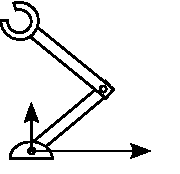
\includegraphics[width=0.27\textwidth]{figs/fwk2dofarm}
    \def\svgwidth{0.4\textwidth}
    \import{./figs/kinematics/}{fwk2dofarm.pdf_tex}
    \caption{A simple 2-DOF arm.}\label{fig:fwk2dofarm}
\end{figure}

Consider the robot arm in \cref{fig:fwk2dofarm}; it is mounted to a table, and is composed of two links and two joints. Let the length of the first link be $l_1$ and the length of the second link be $l_2$. You could specify the position of the link closer to the table by the angle $\alpha$ and the angle of the second link relative to the first link using the angle $\beta$.
Therefore, in this case $q = [\alpha, \beta]^T$.
Our goal is to calculate the position $[x, y]^T$ and orientation $\theta$ of the end-effector; consequently, $f$ will map to $r = [x, y, \theta]^T$.

Let's now calculate the position $P_1 = (x_1, y_1)$ of the joint between the first and the second link using simple trigonometry:
%
\begin{eqnarray}\label{eq:cosxl1}
x_1 &=&l_1 \cos \alpha \nonumber \\
y_1 &=&l_1 \sin \alpha
\end{eqnarray}
%
Similarly, the position of the end-effector $P_2 = (x_2, y_2)$ is given by:
%
\begin{eqnarray}
x_2&=&x_1 + l_2 \cos(\alpha+\beta) \nonumber \\
y_2&=&y_1 + l_2 \sin(\alpha+\beta)
\end{eqnarray}
%
For what concerns the orientation of the arm's end-effector $\theta$, we know it is just the sum of $\alpha+\beta$.
Altogether, the configuration $r$ of the end-effector is given by:
%
\begin{eqnarray}\label{eq:fwk2dofarm}
x&=&l_1 \cos \alpha + l_2 \cos(\alpha+\beta) \nonumber \\
y&=&l_1 \sin \alpha + l_2 \sin(\alpha+\beta) \\
\theta&=& \alpha + \beta \nonumber
\end{eqnarray}
%
The above equations represent \textsl{the forward kinematic equations} of the robot---as they relate its control parameters $ \alpha$ and $\beta$ (also known as joint configuration) to the pose of its end-effector in the local coordinate system spanned by $x$ and $ y$ with the origin at the robot's base.
Note that both $\alpha$ and $\beta$ shown in the figure are positive: both links rotate around the $z-$axis. Using the right-hand rule, the direction of positive angles is defined to be counter-clockwise.

The \emph{configuration space}\index{Configuration space}\index{C-Space (Configuration space)} of the robot---i.e. the set of angles each actuator can be set to---is given by $ 0 < \alpha < \pi $ as it is not supposed to run into the table, and $ -\pi < \beta < \pi$.
The configuration space is given with respect to the robot's joints and allows us to use the forward kinematics equations to calculate the \emph{workspace}\index{Workspace} of the robot, i.e. the physical space it can move to.
This terminology will be identical for mobile robots. An example of configuration and workspace for both a manipulator and a mobile robot is shown in \cref{fig:holonomy}.

% As shown in \cref{fig:fwk2dofarm}, the orientation of the arm's end-effector is given by $\alpha+\beta$.
We can now write down  a transformation that includes a rotation around the z-axis:
\begin{equation}
\label{eq:2armtrans}
f(q) = \left[\begin{array}{cccc}cos_{\alpha\beta} & -sin_{\alpha\beta} &  0 & \cos_{\alpha\beta}l_2+\cos\alpha l_1\\
                        sin_{\alpha\beta} & cos_{\alpha\beta} & 0 & \sin_{\alpha\beta}l_2+\sin\alpha l_1\\
                                                0 & 0 & 1 & 0\\
                                                0 & 0 & 0 & 1\end{array}\right]
\end{equation}
The notation $sin_{\alpha\beta}$ and $cos_{\alpha\beta}$ are shorthand for $sin(\alpha+\beta)$ and $cos(\alpha+\beta)$, respectively.
%
This transformation now allows us to transform from the robot's base to the robot's end-effector configuration $r = [x, y, \theta]^T$ as a function of the joint configuration $q = [\alpha, \beta]^T$.
This transformation will be helpful if we want to calculate suitable joint angles in order to reach a certain pose (i.e., inverse kinematics) or if we want to convert measurements taken relative to the end-effector back into the base's coordinate system (e.g., when we have sensors mounted on the end effector whose output needs to be mapped back to the world reference frame).

\subsection{Forward Kinematics of a Differential Wheels Robot}\label{sec:kinematics:fwk:mobile}

Whereas the pose of a robotic manipulator is uniquely defined by its joint angles---which can be made available using encoders in almost real-time, see \cref{sec:sensors:encoders}---this is not the case for a mobile robot.
Here, the encoder values simply refer to wheel orientation and need to be integrated over time in order to assess the robot's position with respect to the worlds frame of reference; as we will later see, this is a great source of uncertainty.
What complicates matters is that for so-called \emph{non-holonomic} systems, it is not sufficient to simply measure the distance that each wheel traveled, but also when each movement was executed.

\begin{figure}[!t]
    \small
    \centering
    % 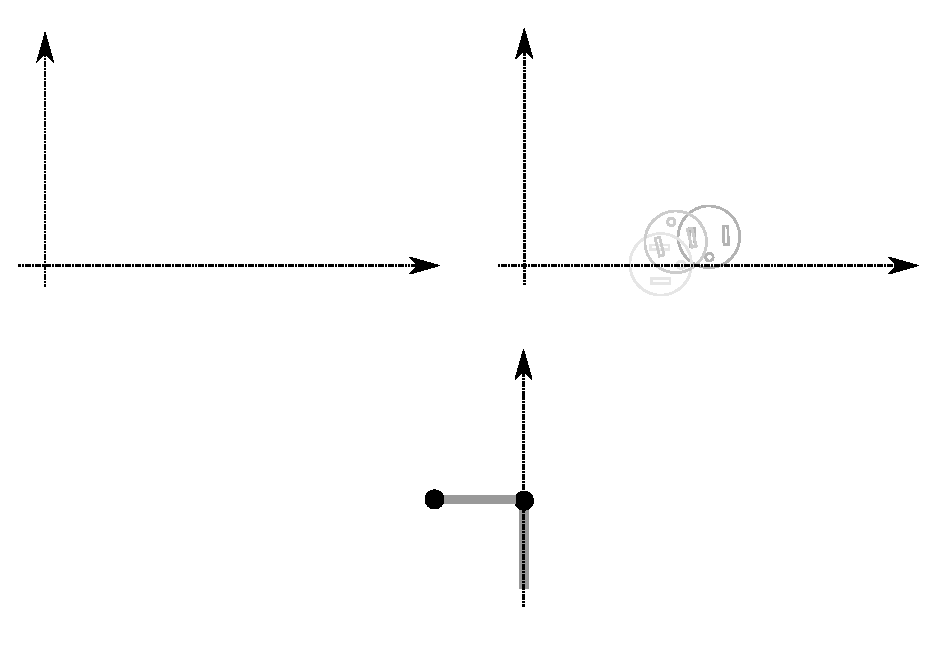
\includegraphics[width=0.95\textwidth]{figs/holonomy.png}
    \def\svgwidth{\textwidth}
    \import{./figs/kinematics/}{holonomy.pdf_tex}
    \caption{Configuration or joint space (left) and workspace or operational space (right) for a non-holonomic mobile robot (top) and a holonomic manipulator (bottom). Closed trajectories in configuration space result in closed trajectories in the workspace if the robot's kinematics is holonomic.}
    \label{fig:holonomy}
\end{figure}

A system is non-holonomic\index{Non-holonomic}\index{Holonomic} when closed trajectories in its configuration space may not have it return to its original state (reminder: the configuration or joint space space of a two-link robotic arm is spanned by the possible values of each angle).
A simple arm is holonomic because each joint position corresponds to a unique position in space:
going through whatever trajectory that comes back to the starting point in configuration space, will put the robot's end-effector at the exact same position in operational space.
A train on a track is holonomic: moving its wheels backwards by the same amount they have been moving forward brings the train to the exact same position in space.
A car and a differential-wheel robot are non-holonomic vehicles: performing a straight line and then a right-turn leads to the same amount of wheel rotation than doing a right turn first and then going in a straight line; however getting the robot to its initial position requires not only to rewind both wheels by the same amount, but also getting their relative speeds right.
The configuration and corresponding workspace trajectories for a non-holonomic and a holonomic robot are shown in \cref{fig:holonomy}.
Here, a robot first moves on a straight line, i.e. both wheels turn an equal amount.
Then, the left wheel remains fixed and only the right wheel turns forward.
Then, the right wheel remain fixed and the left wheel turns backward.
Finally, the right wheel turns backward, arriving at the initial encoder values (zero).
Yet, the robot does not return to its origin. Performing a similar trajectory in the configuration space of a two-link manipulator instead, lets the robot return to its initial position.

It should be clear by now that for a mobile robot, not only traveled distance per wheel matters, but also the \textsl{speed} of each wheel as a function of time.
Interestingly however, this information was not required to uniquely determine the pose of a manipulating arm.
Let's introduce the following conventions.
We will establish a world coordinate system $\{I\}$---which is known as the inertial frame by convention (see \cref{fig:mobilerobot}).
We establish a coordinate system $\{R\}$ on the robot and express the robot's speed $^R\dot{\xi}$ as a vector $ ^R\dot{\xi}=[^R\dot{x}, ^R\dot{y}, ^R\dot{\theta}]^T$. Here $^R\dot{x}$ and $^R\dot{y}$ correspond to the speed along the $x$ and $y$ directions in $\{R\}$, whereas $^R\dot{\theta}$ corresponds to the rotation velocity around the $z-$axis, that you can imagine to be sticking out of the ground.
We denote speeds with dots over the variable name, as speed is simply the derivative of distance.
Now, let's think about the robot's position in $\{R\}$. It is always zero, as the coordinate system is fixed on the robot itself.
Therefore, velocities are the only interesting quantities in this coordinate system and we need to understand how velocities in $\{R\}$ map to positions in $\{I\}$, which we denote by $^I\xi=[^Ix, ^Iy, ^I\theta]^T$. These coordinate systems are shown in \cref{fig:mobilerobot}.

\begin{figure}[htb!]
    \centering
    % 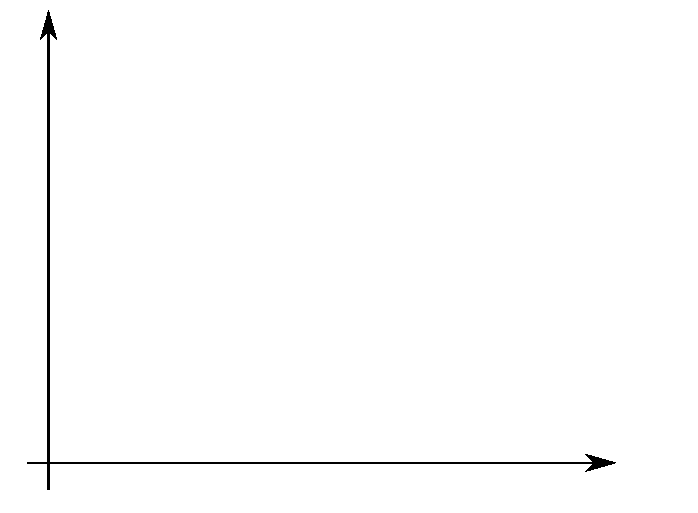
\includegraphics[width=0.85\textwidth]{figs/mobilerobot.png}
    \def\svgwidth{0.85\textwidth}
    \import{./figs/kinematics/}{mobilerobot.pdf_tex}
    \caption{Mobile robot with local coordinate system \{R\} and world frame \{I\}. The arrows indicate the positive direction of position and orientation vectors.}
    \label{fig:mobilerobot}
\end{figure}

Notice that the positioning of the coordinate frames and their orientation are arbitrary. Here, we choose to place the coordinate system in the center of the robot's axle and align $^Rx$ with its default driving direction.
In order to calculate the robot's position in the inertial frame, we need to first find out how speed in the robot coordinate frame maps to speed in the inertial frame.
This can be done again by employing trigonometry. There is only one complication: a movement into the robot's $x-$axis might lead to movement along both the $x-$axis and the $y-$axis of the world coordinate frame ${I}$. By looking at \cref{fig:mobilerobot}, we can derive the following components to $\dot{x}_I$. First,
\begin{equation}
\dot{x}_{I,x}=cos(\theta) \dot{x}_R.
\end{equation}

There is also a component of motion coming from $ \dot{y}_R$ (ignoring the kinematic constraints for now, see below).  For negative $ \theta$, as in \cref{fig:mobilerobot}, a move along $y_R$ would let the robot move into positive $ X_I$ direction. The projection from $ \dot{y}_R$ is therefore given by
\begin{equation}
\dot{x_{I,y}}=-sin(\theta)\dot{y_R}.
\end{equation}
We can now write
\begin{equation}
\dot{x_I}=cos(\theta) \dot{x_R} - sin(\theta) \dot{y_R}.
\end{equation}
Similar reasoning leads to:
\begin{equation}
\dot{y_I}=sin(\theta) \dot{x_R} + cos(\theta) \dot{y_R}
\end{equation}
and
\begin{equation}
\dot{\theta_I}=\dot{\theta_R}
\end{equation}
which is the case because both robot's and world coordinate system share the same z-axis in this example. We can now conveniently write
\begin{equation}
\dot{\xi_I}=^I_RT(\theta)\dot{\xi_R}
\end{equation}
with
\begin{equation}
^I_RT(\theta)=\left[\begin{array}{ccc}
cos(\theta) & -sin(\theta) & 0 \\
sin(\theta) & cos(\theta) & 0 \\
0 & 0 & 1\end{array}\right]
\end{equation}

We are now left with the problem of how to calculate the speed $ \dot{\xi_R}$ in robot coordinates. For this, we make use of the \emph{kinematic constraints}\index{Kinematic constraints} of the robotic wheels.
For a standard wheel in an ideal case scenario, the kinematic constraints are that every rotation of the wheel leads to strictly forward or backward motion and does not allow side-way motion or sliding. We can therefore calculate the forward speed of a wheel $ \dot{x}$ using its rotational speed $ \dot{\phi}$ (assuming the encoder value/angle is expressed as $ \phi$) and radius $ r$ by
\begin{equation}
\dot{x}=\dot{\phi}r.
\end{equation}
This becomes apparent when considering that the circumference of a wheel with radius $r$ is $2\pi r$. The distance a wheel rolls when turned by the angle $ \phi$ (in radians) is therefore $ x=\phi r$, see also \cref{fig:wheelrotation}, right. Taking the derivative of this expression on both sides leads to the above expression.

\begin{figure}[htb!]
    \centering
    % 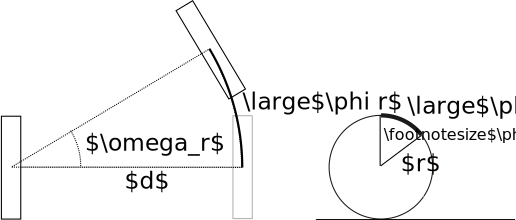
\includegraphics[width=0.9\textwidth]{figs/wheelrotation.png}
    \def\svgwidth{\textwidth}
    \import{./figs/kinematics/}{wheelrotation_2.pdf_tex}
    \caption{Left: Differential wheel robot pivoting around its left wheel first and its right wheel next. For infinitesimal motion, it is possible to decouple left and right wheel to simplify computation of the forward kinematics. Right: A wheel with radius $r$ moves by $\phi r$ when rotated by $\phi$ degrees.}
    \label{fig:wheelrotation}
\end{figure}

How each of the two wheels in our example contributes to the speed of the robot's center---where its coordinate system is anchored---requires the following trick: we calculate the contribution of each individual wheel while assuming all other wheels remaining un-actuated (see \cref{fig:wheelrotation}, left).
In this example, the left wheel will move of $r \phi_l$, and the right wheel will move of $r \phi_r$, which in the space of velocities will become $r\dot{\phi_l}$ and $r\dot{\phi_r}$ respectively.
Then, the distance traveled by the center point is exactly half of that traveled by each individual wheel, assuming the non-actuated wheel rotating around its ground contact point (\cref{fig:wheelrotation}). We can therefore write:
\begin{equation}
\dot{x_R}=\frac{1}{2}\left( r\dot{\phi_l} + r\dot{\phi_r} \right)=\frac{r\dot{\phi_l}}{2}+\frac{r\dot{\phi_r}}{2}
\end{equation}
given the speeds $ \dot{\phi_l}$ and $ \dot{\phi_r}$ of the left and the right wheel, respectively.

\begin{mdframed}
Think about how the robot's speed along its y-axis is affected by the wheel speed given the coordinate system in the drawing above. Think about the kinematic constraints that the standard wheels impose.
\end{mdframed}

Hard to believe at first, but the speed of the robot along its y-axis is always zero. This is because the constraints of the standard wheel tell us that the robot can never slide.
We are now left with calculating the rotation of the robot around its z-axis. This rotation can be seen when imaging the robot's wheels spinning in opposite directions. Then the robot does not move forward, but spins in place.
We will again consider each wheel independently. Assuming the left wheel to be non-actuated, spinning the right wheel forwards will lead to counter-clockwise rotation. Given an axle diameter (distance between the robot's wheels) $d$, we can now write
\begin{equation}
\omega_r d = \phi_r r
\end{equation}
with $\omega_r$ the angle of rotation around the left wheel (\cref{fig:wheelrotation}, left). Taking the derivative on both sides yields speeds and we can write
\begin{equation}
\dot{\omega_r} = \frac{\dot{\phi_r} r}{d}
\end{equation}
Adding the rotation speeds up (with the one around the right wheel being negative based on the right-hand grip rule), leads to:
%
\begin{equation}
\dot{\theta}=\frac{\dot{\phi_r} r}{d}-\frac{\dot{\phi_l} r}{d}
\end{equation}
%
Putting it all together, we can finally write:

\begin{equation}\label{eq:kinematics:forward:mobile}
\left[\begin{array}{c} \dot{x_I}\\\dot{y_I}\\\dot{\theta}\end{array}\right]=\left[\begin{array}{ccc}
cos(\theta) & -sin(\theta) & 0 \\
sin(\theta) & cos(\theta) & 0 \\
0 & 0 & 1\end{array}\right]\left[\begin{array}{c}\frac{r\dot{\phi_l}}{2}+\frac{r\dot{\phi_r}}{2}\\0\\\frac{\dot{\phi_r} r}{d}-\frac{\dot{\phi_l} r}{d}\end{array}\right]
\end{equation}

\subsubsection{From Forward Kinematics to Odometry}

\cref{eq:kinematics:forward:mobile} only provides us with the relationship between the robot's wheel speed and its speed in the inertial frame.
Calculating its actual pose in the inertial frame is known as \emph{odometry}\index{Odometry}. Technically, it requires integrating \cref{eq:kinematics:forward:mobile} from 0 to the current time $T$.
As this is not possible but for very special cases, one can approximate the robot's pose by summing up speeds over discrete time intervals, or more precisely:
\begin{equation}
\left[\begin{array}{c} {x_I}(T)\\{y_I}(T)\\{\theta}(T)\end{array}\right]=
\int_0^T \left[\begin{array}{c} \dot{x_I}(t)\\\dot{y_I}(t)\\\dot{\theta}(t)\end{array}\right] dt \approx
\sum_{k=0}^{k=T}\left[\begin{array}{c} \Delta{x_I}(k)\\\Delta{y_I}(k)\\\Delta{\theta}(k)\end{array}\right]\Delta t
\end{equation} which can be calculated incrementally as
\begin{equation}\label{eq:odometry}
x_I(k+1)=x_I(k)+\Delta x (k) \Delta t
\end{equation}
using $\Delta x(k) \approx \dot{x_I}(t)$ and similar expressions for $y_I$ and $\theta$. Note that \cref{eq:odometry} is just an approximation. The larger $\Delta t$ becomes, the more inaccurate this approximation becomes as the robot's speed might change during the interval.

\begin{mdframed}
\noindent Don't let the notion of an integral worry you! As robots' computers are fundamentally discrete, integrals usually turn into sums, which are nothing than for-loops.
\end{mdframed}

\subsection{Forward kinematics of Car-like steering}\label{sec:kinematics:fwk:car}

Differential wheel drives are very popular in mobile robotics as they are very easy to build, maintain, and control.
Although not holonomic, a differential drive can approximate the function of a fully holonomic robot by first driving on the spot to achieve the desired heading and then driving straight.
Drawbacks of the differential drive are its reliance on a caster wheel, which performs poorly at high speeds, and difficulties in driving straight lines as this requires both motors to drive at the exact same speed.

These drawbacks are mitigated by car-like mechanisms, which are driven by a single motor and can steer their front wheels. This mechanism is known as ``Ackermann steering''. \index{Ackermann steering}
Ackermann steering should not be confused with ``turntable'' steering \index{Turntable steering} where the front wheels are fixed on an axis with central pivot point.
Instead, each wheel has its own pivot point and the system is constrained in such a way that all wheels of the car drive on circles with a common center point, avoiding skid.
As the Ackermann mechanism lets all wheels drive on circles with a common center point, its kinematics can be approximated by those of a tricycle with rear-wheel drive, or even simpler by a bicycle. This is shown in \cref{fig:ackermann}.

\begin{figure}[htb!]
    \centering
    % 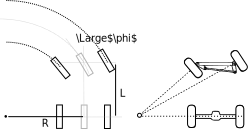
\includegraphics[width=0.9\textwidth]{figs/ackermann.png}
    \def\svgwidth{0.9\textwidth}
    \import{./figs/kinematics/}{ackermann.pdf_tex}
    \caption{Left: Kinematics of car-like steering and the equivalent bicycle model. Right: Mechanism of an Ackermann vehicle.}
    \label{fig:ackermann}
\end{figure}

Let the car have the shape of a box with length $L$ between rear and front axis. Let the center point of the common circle described by all wheels be distance $ R$ from the car's longitudinal center line. Then, the steering angle $ \phi$ is given by

\begin{equation}\label{eq:ackermann}
\tan \phi = \frac{L}{R}
\end{equation}

The angles of the left and the right wheel, $ \phi_l$ and $ \phi_r$ can be calculated using the fact that all wheels of the car rotate around circles with a common center point. With the distance between the two front wheels $l$, we can write:
\begin{eqnarray}
\frac{L}{R-l/2}&=\tan{(\phi_r)} \nonumber \\
\frac{L}{R+l/2}&=\tan{(\phi_l)}
\end{eqnarray}
This is important, as it allows us to calculate the resulting wheel angles resulting from a specific angle $\phi$ and test whether they are within the constraints of the actual vehicle.

Assuming the wheel speed to be $\dot{\omega}$ and the wheel radius $r$, we can calculate the speeds in the robot's coordinate frame as:
\begin{eqnarray}
\dot{x}_r&=&\dot{\omega}r \nonumber \\
\dot{y}_r&=&0\\
\dot{\theta}_r&=&\frac{\dot{\omega}r\tan\phi}{L} \nonumber
\end{eqnarray}
using (\ref{eq:ackermann}) to calculate the circle radius $R$.

\subsection{The Denavit-Hartenberg notation}\label{sec:kinematics:fwk:dh}

So far, we have considered the forward kinematics of wheeled mechanisms and simple arms and derived relationships between actuator parameters and velocities using basic trigonometry.
In the case of multi-link arms (which is the vast majority of robot manipulators in existence), the approach detailed in \cref{sec:kinematics:fwkarm} is difficult to scale, and alternative solutions are needed.
Interestingly, we can think of the forward kinematics as a chain of homogeneous transformations with respect to a coordinate system mounted at the base of a manipulator or a fixed position in the room.
Deriving these transformations can be confusing and can be facilitated by following a ``recipe'' such as the one conceived by Denavit and Hartenberg in $1955$ (see \cite{hartenberg1955kinematic} and \cite{craig2009introduction}).
The so-called Denavit-Hartenberg (DH)\index{Denavit-Hartenberg parameters} representation has since evolved as a \textsl{de-facto} standard.

A manipulator consists of a series of typically rigid links that are connected by joints.
In the vast majority of cases, a joint can either be revolute (i.e. change its angle/orientation) or prismatic (i.e. change its length).
Knowing the robot's kinematic properties (e.g. the length of all rigid links, similarly to $l_1$ and $l_2$ in \cref{fig:fwk2dofarm}), the pose of its end-effector is fully described by its joint configuration (angle for revolute joints, length for prismatic joints).

%In industrial manipulators, the number of joints is usually equal to the degrees of freedom of the manipulator. As most manipulators are holonomic, the forward kinematics allow you---unlike on non-holonomic wheeled platforms---to directly relate absolute positions of joints with absolute positions in Cartesian space. It is also possible to derive equations that relate the speed of the joints to speed in Cartesian space. Like for wheeled platforms, this can be achieved via a Jacobian matrix.  At certain positions, the mapping provided by the Jacobian is not invertible, i.e., some velocities in Cartesian space are unachievable. These points are called singularities.

\screencast{http://youtu.be/rA9tm0gTln8}{denavithartenberg}

\begin{figure}[!t]
    \centering
    % 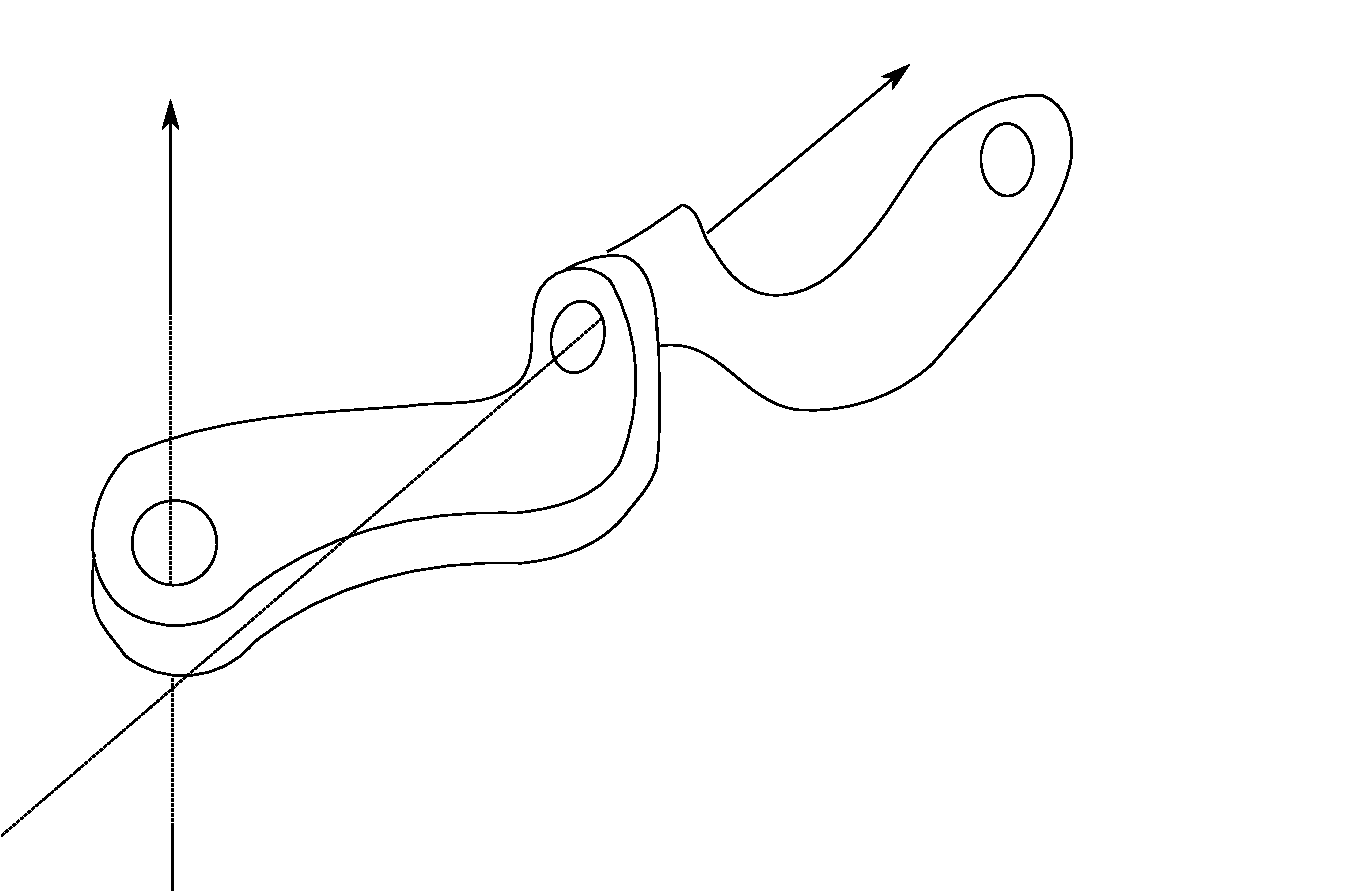
\includegraphics[width=\textwidth]{figs/denavit-hartenberg.png}
    \def\svgwidth{\textwidth}
    \import{./figs/kinematics/}{denavit-hartenberg.pdf_tex}
    \caption{Example of selected Denavit-Hartenberg parameters for three sequential revolute joints. The z-axes of joint $i$ and $i+1$ are parallel, which results in $\alpha_i = 0$.}
    \label{fig:denavit}
\end{figure}

In order to use the DH-convention, we first need to define a coordinate system at each joint. With reference to \cref{fig:denavit}, we choose the $z-$axis to be the axis of rotation for a revolute joint and the axis of translation for a prismatic joint.
We can now find the common normal between the $z-$axes of two subsequent joints, i.e. a line that is orthogonal to each $z-$axis and intersects both.
With the direction of the $x-$axis at the base arbitrary, subsequent $x-$axes are chosen such that they lie on the common normal shared between two joints.
Whereas the direction of the $z-$axis is given by the positive direction of rotation (right-hand rule), the $x-$axis points away from the previous joint.
This allows defining the $y-$axis using the right-hand rule.
Note that these rules, in particular the requirement that $x$-axes lie along the commom normal, might result in coordinate systems with their origins outside the joint: this is not relevant as the kinematics of a manipulator is a mathematical representation that needs to represent the geometric and kinematic properties of the robot, and does not need to bear any physical correspondence.
%
The transformation between two joints is then fully described by the following four parameters:
\begin{enumerate}
\item The length $r$ (sometimes, $a$ is used) of the common normal between the $z$-axes of two joints $i$ and $i-1$ (link length).
\item The angle $ \alpha$ between the z-axes of the two joints with respect to the common normal (link twist), i.e. the angle between the old and the new $z$-axis, measured about the common normal.
\item The distance $d$ between the joint axes (link offset), i.e. the offset along the previous $z$-axis to the common normal.
\item The rotation $ \theta$ around the common axis along which the link offset is measured (joint angle), i.e. the angle from the old $x$-axis to the new $x$-axis, about the previous $z$-axis.
\end{enumerate}

Two of the above D-H parameters describe the link between the joints, and the other two describe the link's connection to a neighboring link.
Depending on the link/joint type, these numbers are fixed by the specific mechanical instance of the robot or can be controlled.
For example, in a revolute joint $ \theta$ is the varying joint angle, while all other quantities are fixed.  Similarly, for a prismatic joint $d$ is the joint variable. An example of two revolute joints is shown in \cref{fig:denavit}.

The final coordinate transform from one link ($i-1$) to another ($i$) can now be constructed by concatenating the four steps above, which are nothing but a series of rotations and translations, one for each DH parameter:
%
\begin{equation}\label{eq:kinematics:dh:composition}
_{n-1}^nT=T_z'(d_n) R_z'(\theta_n) T_x(r_n)  R_x(\alpha_n)
\end{equation}
with
\begin{equation}
T_z'(d_n)=
\left[ \arraycolsep=2pt%\def\arraystretch{2.2}
\begin{array}{ccc|c}
1 & 0 & 0 & 0\\
0 & 1 & 0 & 0\\
0 & 0 & 1 & d_n\\
\hline
0 & 0 & 0 & 1
\end{array}
\right]
\enskip
R_z'(\theta_n)=\left[ \arraycolsep=2pt%\def\arraystretch{2.2}
\begin{array}{ccc|c}
\cos\theta_n & -\sin\theta_n & 0 & 0\\
\sin\theta_n & \cos\theta_n & 0 & 0\\
0 & 0 & 1 & 0\\
\hline
0 & 0 & 0 & 1
\end{array}
\right]
\end{equation}
and
\begin{equation}
T_x(r_n)=
\left[ \arraycolsep=2pt%\def\arraystretch{2.2}
\begin{array}{ccc|c}
1 & 0 & 0 & r_n\\
0 & 1 & 0 & 0\\
0 & 0 & 1 & 0\\
\hline
0 & 0 & 0 & 1
\end{array}
\right]
\enskip
R_x(\alpha_n)=\left[ \arraycolsep=2pt%\def\arraystretch{2.2}
\begin{array}{ccc|c}
1 & 0 & 0 & 0\\
0 & \cos\alpha_n & -\sin\alpha_n & 0\\
0 & \sin\alpha_n & \cos\alpha_n & 0\\
\hline
0 & 0 & 0 & 1
\end{array}
\right]
\end{equation}
%
These are a translation of $d_n$ along the previous z-axis ($T_z'(d_n)$), a rotation of $\theta_n$ about the previous z-axis ($R_z'(\theta_n)$), a translation of $r_n$ along the new $x$-axis ($T_x(r_n)$)and a rotation of $\alpha_n$ around the new $x$-axis ($R_x(\alpha_n)$).
%
By replacing each element in \cref{eq:kinematics:dh:composition}, the following matrix is created:
\begin{eqnarray}
_{n-1}^nT&=
\left[ \arraycolsep=2pt%\def\arraystretch{2.2}
\begin{array}{ccc|c}
\cos \theta_n & -\sin \theta_n \cos\alpha_n & \sin\theta_n \sin\alpha_n & r_n \cos\theta_n\\
\sin \theta_n & \cos\theta_n \cos\alpha_n & -\cos\theta_n\sin\alpha_n & r_n \sin\theta_n\\
0 & \sin\alpha_n & \cos\alpha_n & d_n \nonumber \\
\hline
0 & 0 & 0 & 1
\end{array}
\right]\\
&=
\left[ \arraycolsep=2pt%\def\arraystretch{2.2}
\begin{array}{c|c}
R & t\\
\hline
0 \quad 0 \quad 0 & 1
\end{array}
\right]
\end{eqnarray}
where $R$ is the $3\times3$ rotation matrix and $t$ is the $3\times1$ translation vector.

Like for any homogeneous transform, the inverse $_{n-1}^nT^{-1}n$ is given by
\begin{equation}
^{n-1}_nT=\left[ \arraycolsep=2pt%\def\arraystretch{2.2}
\begin{array}{c|c}
R^{-1} & -R^{-1}T\\
\hline
0 \quad 0 \quad 0 \quad 1
\end{array}
\right]
\end{equation}
with the inverse of $R$ simply being its transpose, $R^{-1}=R^T$.

Similar to the concatenation of transformations detailed in \cref{sec:kinematics:coordsystems:concatenation}, $_{n-1}^nT$ in \cref{eq:kinematics:dh:composition} can be concatenated with the other transformation matrices relative to the remaining links in order to compute a the full kinematics of the robot arm from the base reference frame up to the end-effector.
% \td{Nikolaus, should we add half a page of text plus a figure to describe this further? I feel they are left hanging without it}
